% % % Set the style for this file:
\pagestyle{standard}

% % % Beginning of the chapter
\chapter{Experimental setup}\label{chapter2}

	% % % Set the style for the first page:
	\thispagestyle{chapter-first-page}
	
	\section{Thermo-mechanical petal}\label{section2.1}
	
		Both ATLAS ITk strip end-caps (Figure \ref{fig2.1} left) are composed by six disks, which individually can hold 32 local support structures called petals (Figure \ref{fig2.1} right). The petal structure is the frame where the end-cap sensors are mounted. It provides the mechanical support needed by the sensors as well as the electronics and cooling services. Each petal holds 9 sensors (Figure \ref{fig2.1} right). 
		In this study we use a thermo-mechanical prototype equipped with dummy electronics modules, blank silicon wafers and mechanical components to be a thermal equivalent to the final structure. As the petal’s design is still being improved, our prototype became quickly “obsolete”. In fact, some key materials for IR studies in the current prototype such as the silicon wafers are not very IR friendly because of their high transmissivity. This makes the employment of non-contact temperature measuring methods really difficult (See Chapter \ref{chapter4}). The new wafers considered for the final design are, however, not transmissive.
				
		\begin{figure}[ht!]
			\centering
			\captionsetup{justification=centering,margin=2cm}
			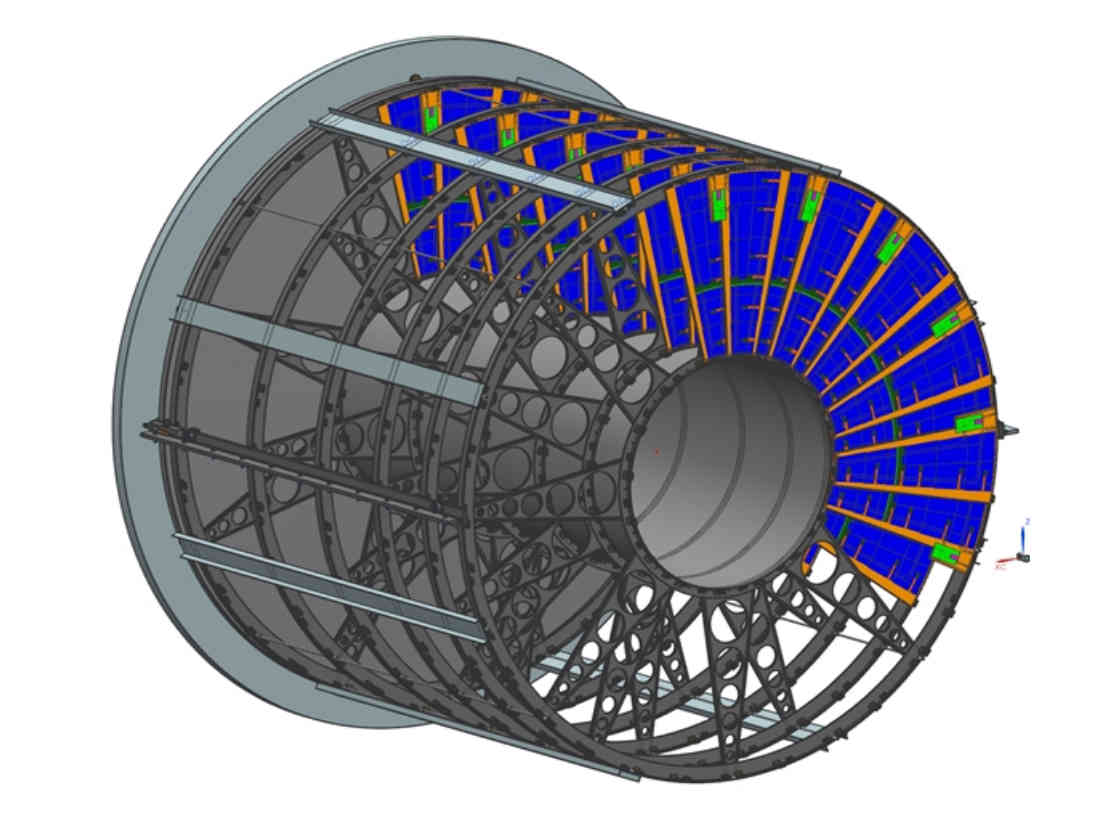
\includegraphics[scale=0.25]{Figures/Chapter02/EndCap.jpg}
			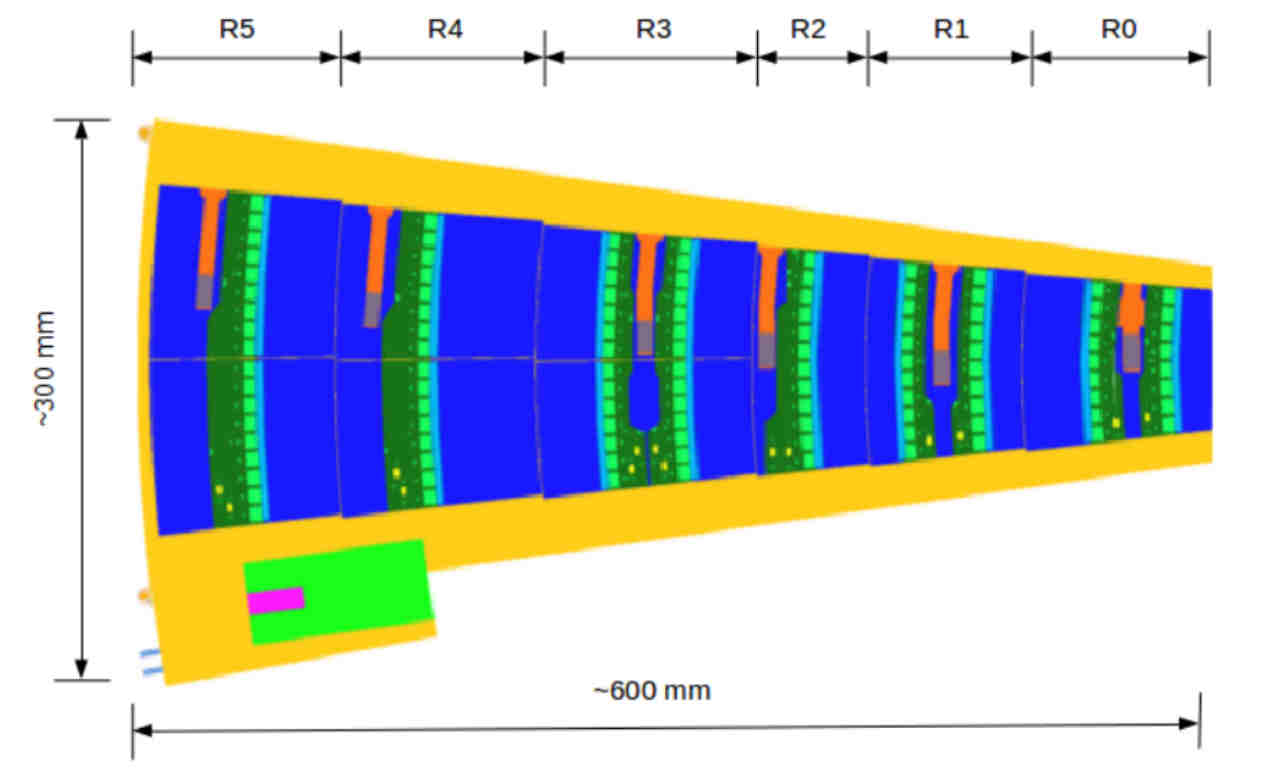
\includegraphics[scale=0.26]{Figures/Chapter02/PetalDesign.jpg}
			\caption{ATLAS strip detector end-cap (left) showing petal structures and a schematic view of the petal showing the 6 different modules (right).}\label{fig2.1}
		\end{figure}
		
		The nine modules of each petal side are glued on the petal core (carbon facesheets) in six subsegments referred to as rings (R0 - R5). Each module contains the following components:
		
		\begin{itemize}
			\renewcommand{\labelitemi}{$\diamond$}
			\item Blank Si, laser cut (320 $\mu$m thick).
			\item FR4 PCBs (200 $\mu$m thick).
			\item Glass ASICs with heater pattern and bonding pads, glued with UV glue, wire-bonded to bare silicon.
			\item Real DC-DC converters, based on commercial LTC360 ASIC on a custom board.
			\item Potentiometer to adjust power input/output.
			\begin{itemize}
			\renewcommand{\labelitemi}{$\bullet$}
				\item Powered through bus tape power lines.
			\end{itemize}
			\item In the case of R0 module: v0 assembly tools, real hybrids, glass ASICs.
		\end{itemize}
		
		In addition, the prototype core was built using real materials with respect to preliminary petal designs (bus tape, honeycomb, Ti V-shaped cooling pipe), real copper power traces, dummy data-lines, and a dummy EoS (not present initially but recently installed) per side. Some of the above-mentioned components can be seen in the Figure \ref{fig2.2}.
		
		\begin{figure}[ht!]
			\centering
			\captionsetup{justification=centering,margin=2cm}
			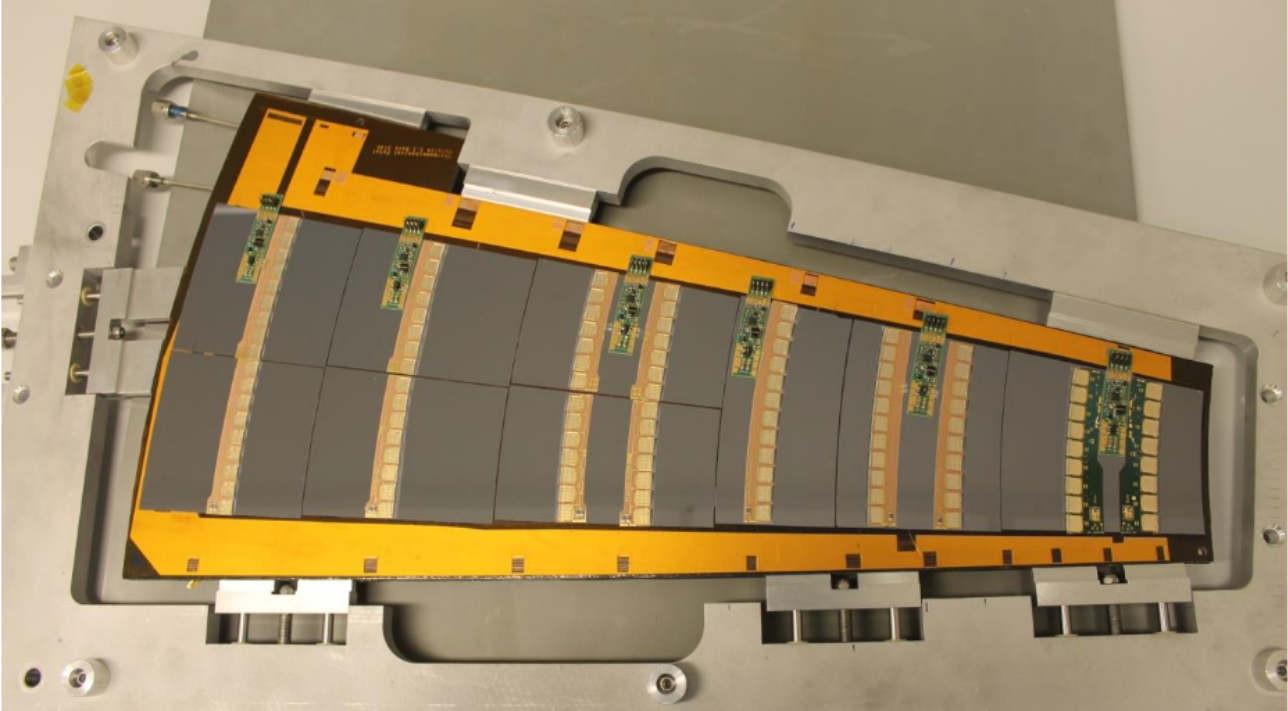
\includegraphics[scale=0.35]{Figures/Chapter02/PetalConstruction.jpg}
			\caption{Thermo-mechanical prototype of the petal  used in the IR measurements.}\label{fig2.2}
		\end{figure}\bigskip
		
	\section{Custom Thermal Chamber. }\label{section2.2}
	
		For the infrared measurements, the thermomechanical petal prototype was placed inside a customised thermal chamber where, on one end, the petal is vertically inserted in a custom rail system (Figure \ref{fig2.3} left) and on the opposite end the IR camera is mounted on a mobile platform that can move horizontally and vertically thanks to an Arduino controlled Gantry System (Figure \ref{fig2.3} right). Temperature and relative humidity (RH) inside the chamber are monitored using three SHT21 sensors connected  to a Raspberry Pi. 
		
		\begin{figure}[ht!]
			\centering
			\captionsetup{justification=centering,margin=2cm}
			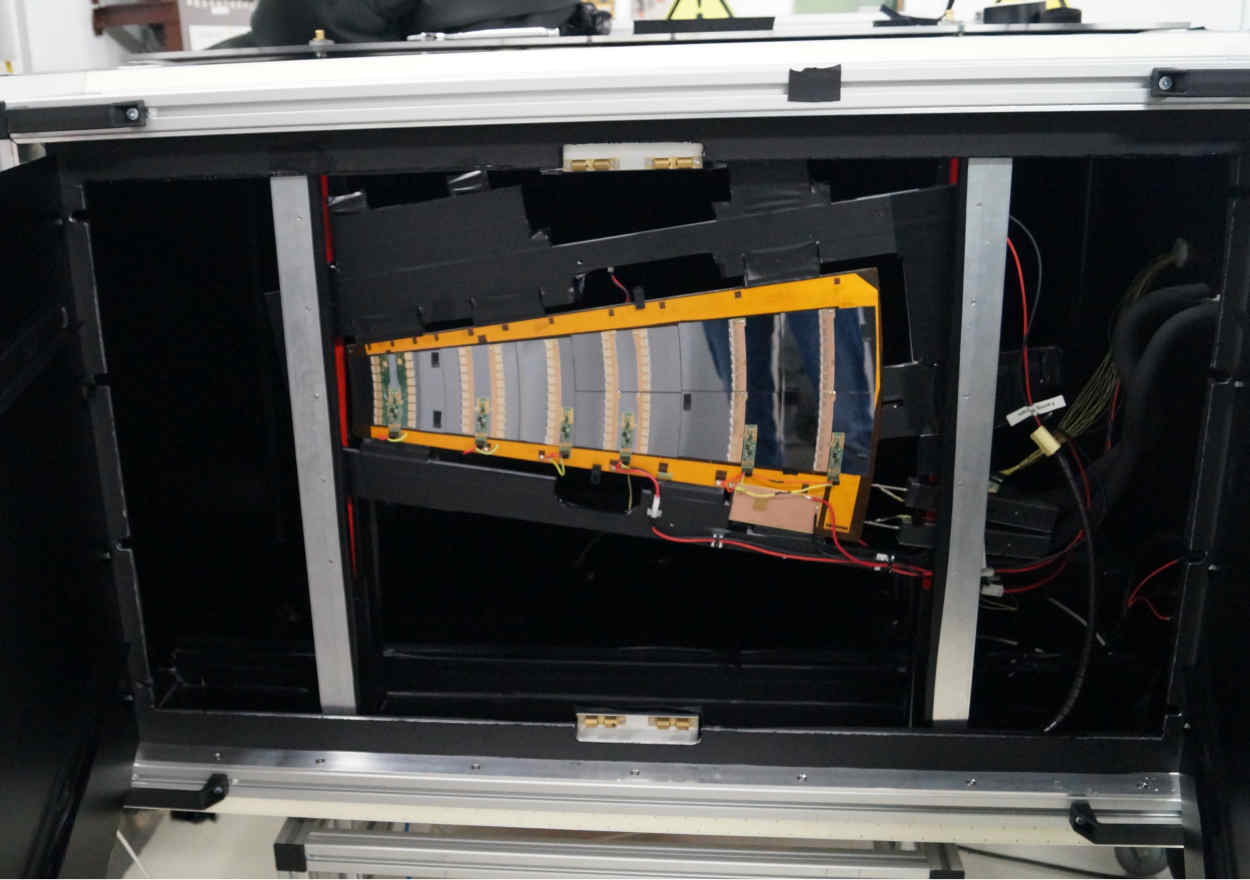
\includegraphics[scale=0.25]{Figures/Chapter02/ChamberBack.jpg}
			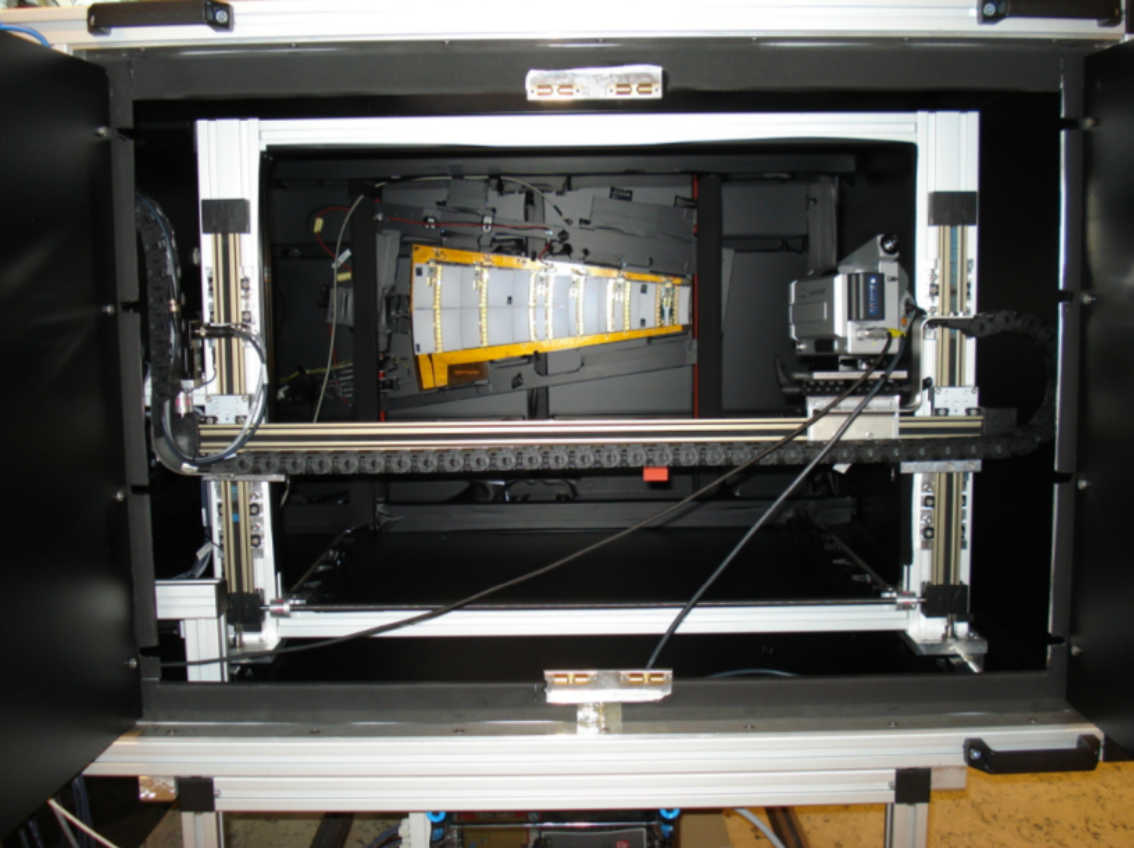
\includegraphics[scale=0.26]{Figures/Chapter02/CamberFront.jpg}
			\caption{Image of both ends of the thermal chamber showing the petal already in place and the IR camera also in position.}\label{fig2.3}
		\end{figure}
		
		The use of the chamber has two main advantages: first, it provides shielding for the object under investigation against external heat sources such as ceiling lamps, computers and other electronic devices used in the setup; second, it is used as an enclosure where we can flush nitrogen in order to reduce the moisture and in doing so preventing condensation from ambient air on the cooled sensors, which would irreversibly damage the prototype. Low RH comes with the additional bonus of reducing the potential absorption of IR radiation in the air path from the target to the IR camera as discussed in Section \ref{section1.1}.
		In order to perform the IR measurements avoiding the heat of IR camera itself to be reflected back by the petal surface\footnote{{\footnotesize This is known as the Narcissus effect and it is an important source of background for the IR measurements if not properly handled.}}, the IR camera is positioned in the chamber in such a way that it faces the petal with an angle of incidence (Figure \ref{fig2.4}).	
		
		\begin{figure}[ht!]
			\centering
			\captionsetup{justification=centering,margin=2cm}
			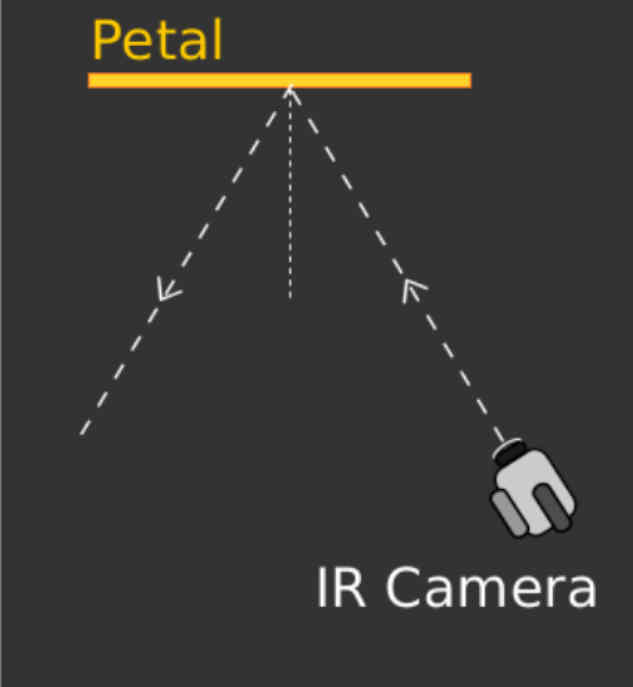
\includegraphics[scale=0.25]{Figures/Chapter02/NarcissusEffect.jpg}
			\caption{The IR camera is placed at some angle with respect to the plane of the petal to avoid the Narcissus effect.}\label{fig2.4}
		\end{figure}\bigskip
		
	\section{IR camera.}\label{section2.3}
	
		For this study a VarioCAM High Resolution (hr) IR camera from InfraTec GmbH was used (Figure \ref{fig2.5}). The VarioCAM$\textregistered$ hr is a thermographic system for the long wave infrared spectral range of 7.5 $\mu$m to 14 $\mu$m (LWIR). The lens images the object scene onto a microbolometer array at a resolution of 640 $\times$ 480 pixels. The electrical signal of the detector arrays is further processed by the internal electronics, which consists in converting the modified pixel resistance due to the incoming radiation into temperature. The electronics also contains all the functions necessary for camera operation, such as activation of the microbolometer array, A/D conversion, offset and gain correction, defective pixel treatment, video and PC interfaces \ref{ref9}.
		
		\begin{table}[ht!]
    		\begin{minipage}[b]{0.4\linewidth}
  				\centering
  				\captionsetup{justification=centering, margin=0.5cm}
  				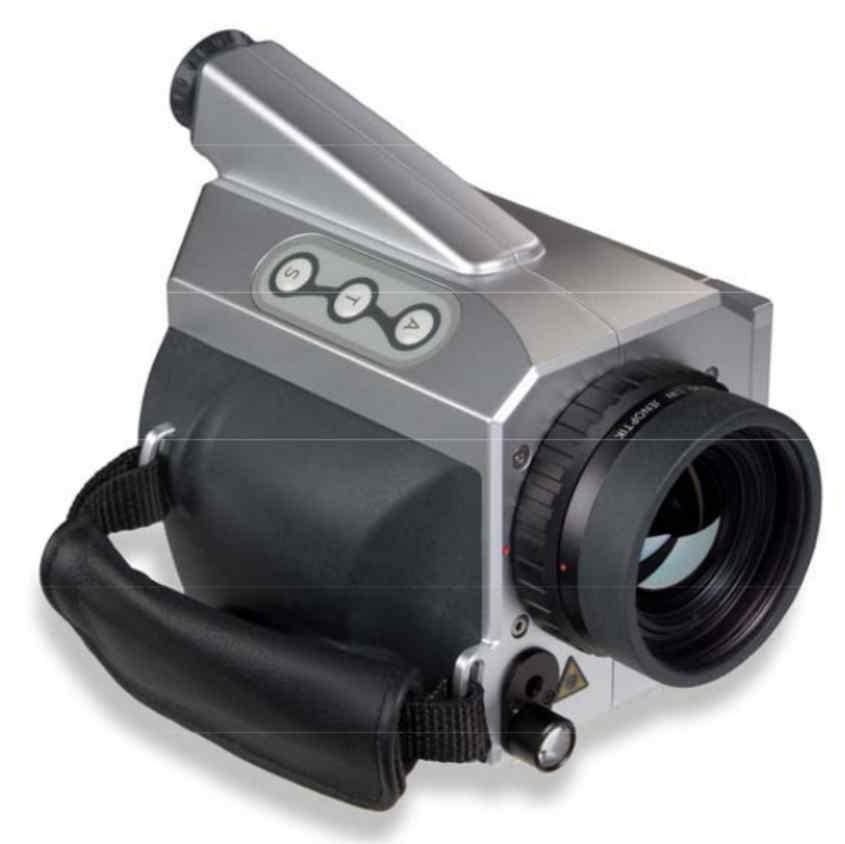
\includegraphics[scale=0.3]{Figures/Chapter02/PictureOfIRCamera.jpg}
  				\captionof{figure}{VarioCAM\textregistered\space hr (640 x 480 pixels) IR camera  from InfraTec \textcopyright\space GmbH.}\label{fig2.5}
    		\end{minipage}
    		\begin{minipage}[b]{0.7\linewidth}
    			\centering
  				\captionsetup{justification=raggedright}
        		\caption{VArioCam hr technical data.}\label{tab2.1}
				\begin{tabular}{p{0.35\linewidth}p{0.35\linewidth}}\hline
					\textbf{Temperature measuring range} & (-40 ... 1.200) $^{\circ}C$, optional $>$ 2.000 $^{\circ}C$ \\ \hline 
					\textbf{Temperature resolution @ 30 $^{\circ}C$} &  better than 0.08 K, up to 0.05 K (premium mode) \\ \hline
					\textbf{Emissivity} & Adjustable from 0.1 to 1.0, in increments of 0.01 \\ \hline
					\textbf{Detector} &  uncooled microbolometer Focal Plane Array \\ \hline
					\textbf{A/D conversion} &  16 bit \\ \hline 
					\textbf{Operation temperature} & (-15 ... 50) $^{\circ}C$ \\ \hline
					\textbf{Humidity during operation and storage} & 5\% to 95\%, non-condensing \\ \hline
					\textbf{Shock resistance} & 25 G, IEC 68-2-29 \\ \hline
				\end{tabular}
    		\end{minipage}
		\end{table}
		
		The camera’s accuracy for temperature measurement (reported by manufacturer) is $\pm 1.5 K$ in the range from 0$^\circ$C to 100$^\circ$C and $\pm2$\% anywhere outside that range. Some additional technical data is presented in Table \ref{tab2.1}.
		
		The data acquisition is performed using the VarioCam hr control software IRBIS$\textregistered$ professional v3.1 (Figure \ref{fig2.6}). Each image is computed as an average of 100 acquisitions regularly taken during five seconds in order to reduce uncertainty due to pixels noise. All thermograms are recorded in units of absolute temperature (K) and emissive power ($W/m^2$) for further offline analysis.
		
		\begin{figure}[ht!]
			\centering
			\captionsetup{justification=centering,margin=2cm}
			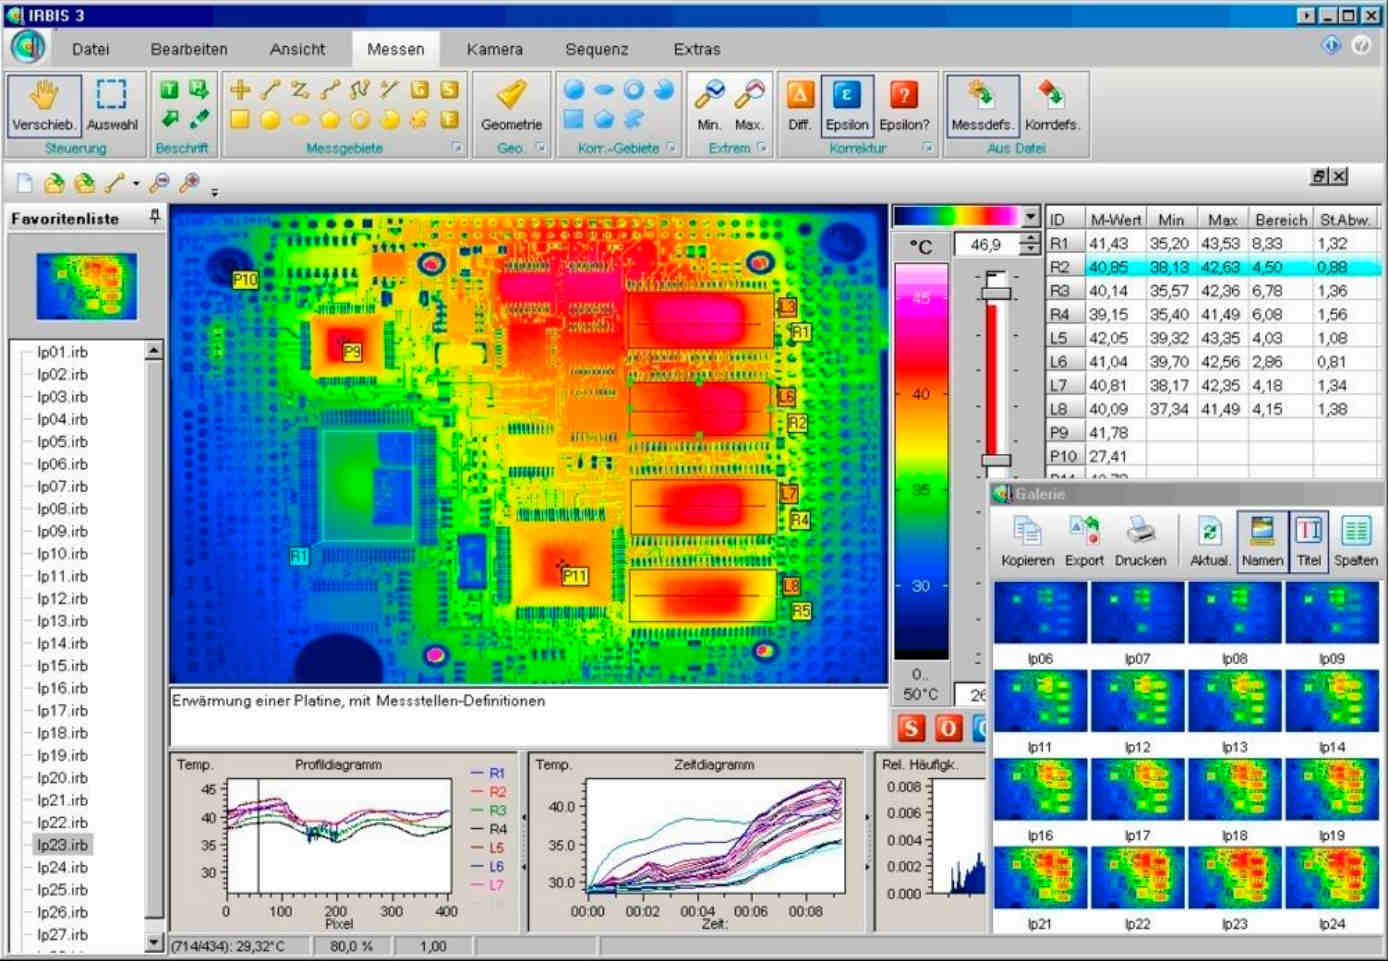
\includegraphics[scale=0.25]{Figures/Chapter02/IRBISimage.jpg}
			\caption{Screenshot of the camera’s control software IRBIS$\textregistered$ 3.1.}\label{fig2.6}
		\end{figure}\bigskip
		
	\section{Setup configuration.}\label{section2.4}
	
		In this study, two thermal tests performed using the setup described below are considered, corresponding to both sides of the petal and measured with the latest experimental configuration. 
		In the following, this will be referred to as “front side test” (unpolished side test) and “back side test” (polished side test) in allusion to the specific side of the petal tested. 
		
		Much of the improvements of the experimental setup came from experiences of preliminary tests when we realized that, for example, the heat from the Gantry system was being reflected on the petal’s surface and registered by the IR camera. Thus, a curtain from an IR opaque black fabric was placed between the petal and the Gantry system (leaving a small hole for the camera lens) to suppress this effect (Figure \ref{fig2.7} right). In addition, other improvements to the chamber’s insulation were made to better control the ambient conditions inside at lower temperatures (Figure \ref{fig2.7} left). 
	
		\begin{figure}[ht!]
			\centering
			\captionsetup{justification=centering,margin=2cm}
			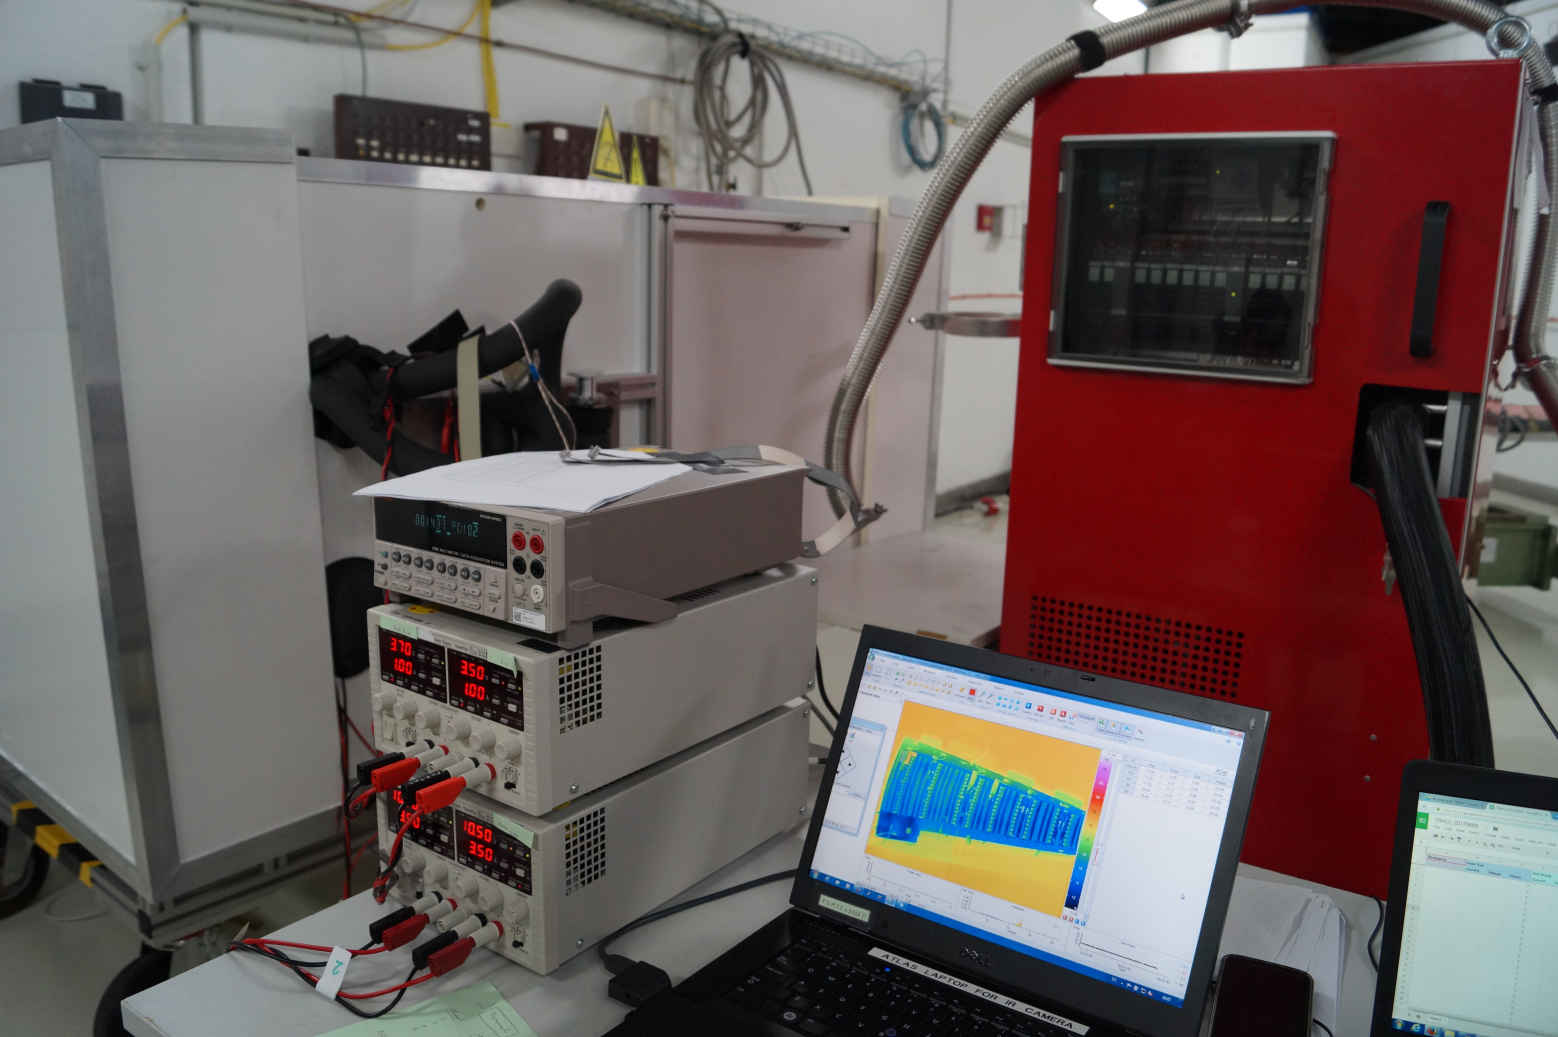
\includegraphics[scale=0.185]{Figures/Chapter02/ExperimentalSetup.jpg}
			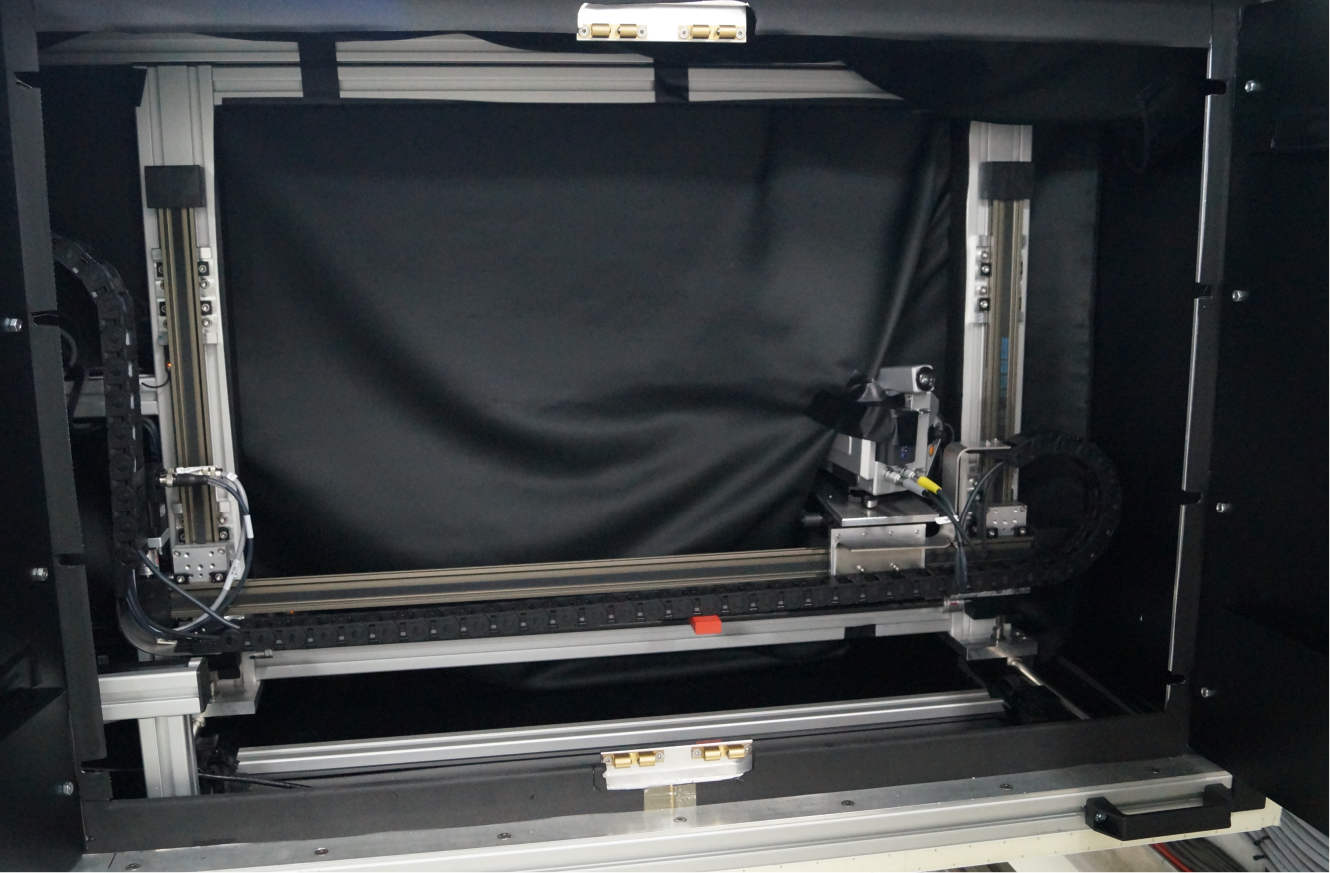
\includegraphics[scale=0.22]{Figures/Chapter02/BlackCurtine.jpg}
			\caption{Experimental setup used for the petal’s thermal tests. Right: a view of the chamber with new insulation, laptop for data acquisition, power supplies and Keithley (next to the laptop) and TRACI (Red box). Left: black curtain installation.}\label{fig2.7}
		\end{figure}
	
		This is particularly important for an accurate estimation of the apparent reflected temperature (See Section \ref{section3.1}). In addition, the DC-DC converters in modules R2 and R3 were covered with 3D-printed caps and black tape due to the fact that their heat created a “halo” of hot air (Figure \ref{fig2.8} right) around them that blurred the thermograms of that area of the petal (Figure \ref{fig2.8} left).
		
		For cooling the petal the \textit{Transportable Refrigeration Apparatus for CO$_{2}$ Investigation} (TRACI) Version 2 (100W) with Lewa pump was used (Figure \ref{fig2.7} left). This was the first time that a themo-mechanical petal prototype was cooled down using by-phase CO$_{2}$ in our setup. Previously, a water-glycol chiller was used, which greatly limited the lowest temperature that we were able to reach.
	
		\begin{figure}[ht!]
			\centering
			\captionsetup{justification=centering,margin=2cm}
			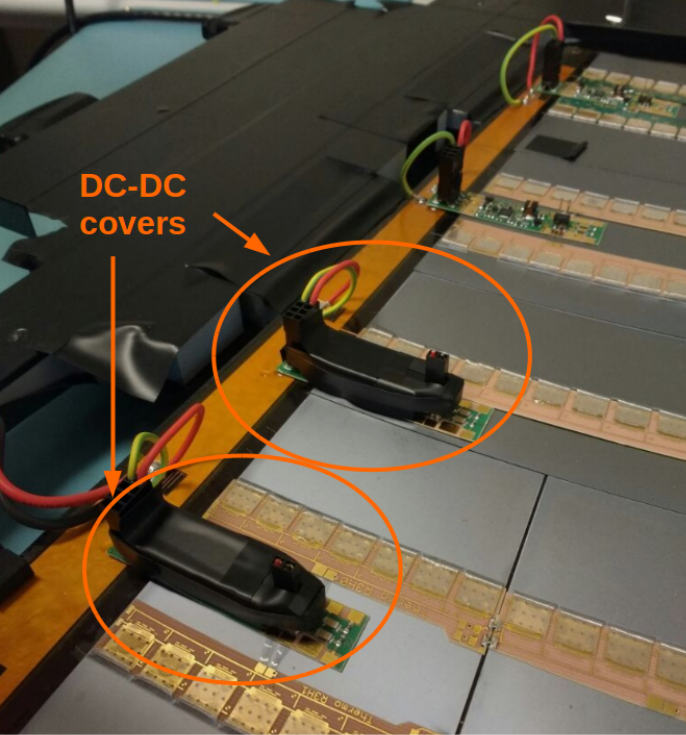
\includegraphics[scale=0.33]{Figures/Chapter02/DCDC_covers.jpg}
			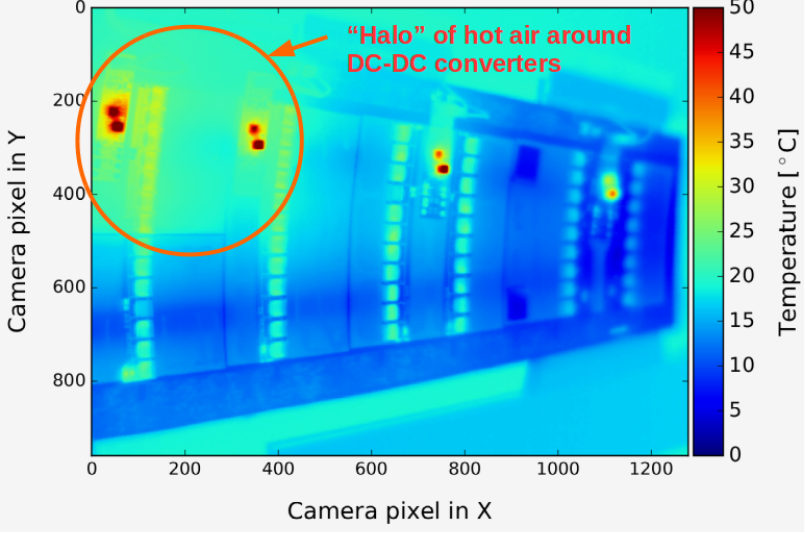
\includegraphics[scale=0.46]{Figures/Chapter02/HaloThermogram.jpg}
			\caption{Unpolished side of the petal showing the DC-DC covers (left) and the thermogram where that “halo” of hot air around them is visible inside the circle (right).}\label{fig2.8}
		\end{figure}
	
		By controlling the CO$_{2}$ pressure in the experiment we were able to adjust the desired temperature working point. Using this method temperatures of near -25$^{\circ}$C were reached.
		
		The petal is equipped with nine dummy circuits simulating the heat emitted by the readout electronics (6 module electronics + 1 EoS) per side. An important aspect for the prototype operation is that the powerboards should have a constant power consumption of $\sim$25W and the EoS $\sim$3W on each side of the petal. To power the powerboards and EoS of both sides, two TTICPX400 power supply units were used. The modules voltage is set to 10.5V and the current to 2.5A. In the case of the EoS the current is set to 1.0A (for both sides) and the voltage to 3V. However, as the resistance of the circuit changes with temperature we had to vary the voltage accordingly to keep the 3W of power consumption constant. For the front side test we did it manually but for the back side test, as part of the Summer Student program, the student involved in the IR project was able to automatize the process by creating a program that automatically varied the voltage input to keep a steady 3W power consumption \ref{ref10}.
		
		In addition, a Keithley 2700 multimeter was used to register the readings from additional PT100 thermocouples using 4 wire sensing and some other important TRACI parameters like, for example, CO$_{2}$ flow, CO$_{2}$ temperature before experiment (petal), CO$_{2}$ temperature after experiment, pressure set-point and pressure of the CO$_{2}$ in the experiment.
		
		The additional thermocouples were placed as follows (for the front side test): 2 on the inlet/outlet pipes (glued), 2 in R3 module silicon surface (maintained by a piece of high emissivity black tape): 1 between the ASICs and 1 in the corner next to R4 (Figure \ref{fig2.9} top). For the four extra thermocouples were placed in R0, R1, R4 and R5 as shown in Figure \ref{fig2.9} (bottom).
		
		\begin{figure}[H]
			\centering
			\captionsetup{justification=centering,margin=2cm}
			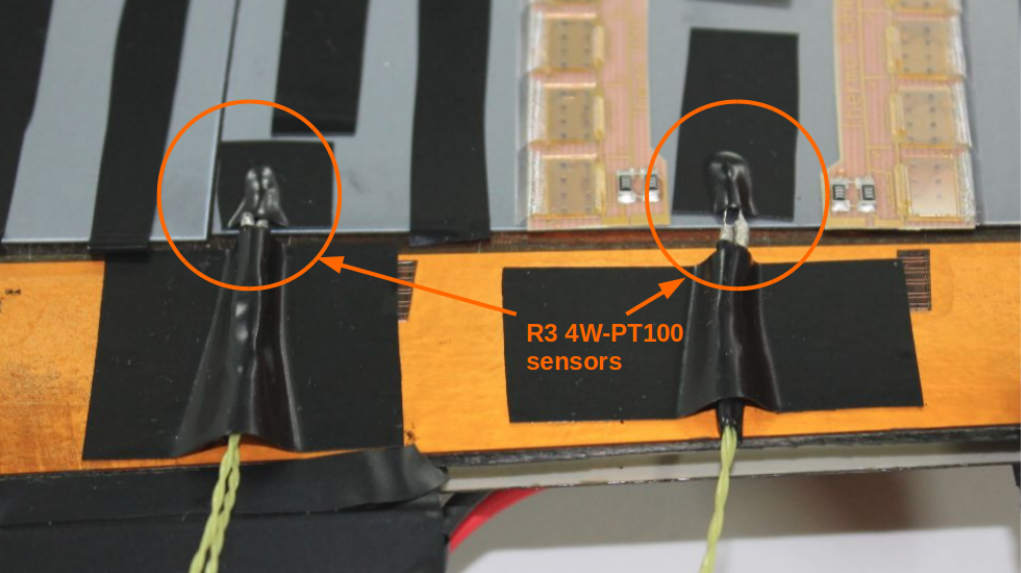
\includegraphics[scale=0.47]{Figures/Chapter02/R3PT100CloseUp.jpg}
			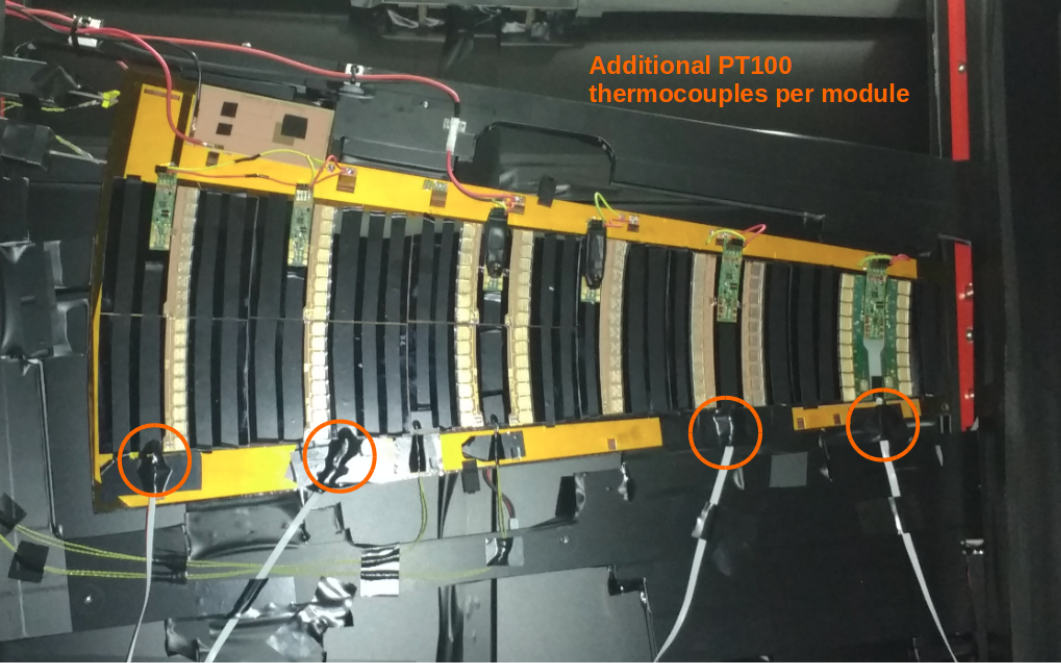
\includegraphics[scale=0.45]{Figures/Chapter02/AdditionalPT100perModule.jpg}
			\caption{Close-up of the unpolished side of the petal showing the 2 PT100 thermocouples attached to R3 module (top). Polished side of the petal ready for the thermal test. The additional PT100 thermocouples placed at each module (except R2) are visible (bottom).}\label{fig2.9}
		\end{figure}
